%!TEX encoding = UTF-8 Unicode
\documentclass{reqenglecture}

\title{Introduction to Software Requirements Engineering}

\subtitle{Part 1: Domain Knowledge}

\author{Björn Regnell}

\date{\vspace{1em}\footnotesize Updated: \today~
\\ License: CC-BY-SA 
\\ \url{https://github.com/bjornregnell/reqeng-book} 
}

%\beamerdefaultoverlayspecification{<+->} %de-comment if you want pause after items

\begin{document}
\maketitle

\begin{frame}
\frametitle{Part 1: Domain Knowledge}
\framesubtitle{Outline}
\tableofcontents
\end{frame}


\LectureOnly{\section{Introduction}}

\begin{Slide}{What is Requirements Engineering (RE)?}

\begin{itemize}
\item RE is focused on the
\begin{itemize}
\item \textbf{features} of software-intensive systems 
\item \textbf{system context}, including users and connected systems
\item \textbf{development context}, including stakeholders' intentions 

\end{itemize}
\item The RE process involves 
\begin{itemize}
\item knowledge-building \hfill research
\item consensus-building \hfill agree
\item decision-making    \hfill choose
\item innovation         \hfill generate ideas
\item communication      \hfill be pedagogical

\end{itemize}
\end{itemize}
\end{Slide}

\begin{Slide}{What is a requirement?}

\begin{itemize}
\item Something \textbf{needed} or \textbf{wanted}.

\item A documented \textbf{representation} of\\something needed or wanted.
\item The word ''requirement'' have different meanings:\\
  must, wish, idea, specific design, rationale, ...

\item The most \textbf{general meaning}:\\
  \textit{any} kind of \textbf{information entity} used in RE

\item You don't always get what you want and you often want things that you don't need...

\end{itemize}
\end{Slide}

\begin{Slide}{Main Activities of RE}

{\vspace{1em}\resizebox{!}{3em}{\hspace{0.5em}{\bf ?}\hspace{0.5em}\WritingHand\hspace{0.5em}\Checkedbox\hspace{0.5em}\LeftScissors}\vspace{0.5em}}

\begin{itemize}
\item The 4 main activities of RE: 
\begin{itemize}
\item \textbf{Elicitation} \hfill learning
\item \textbf{Specification} \hfill representing
\item \textbf{Validation}  \hfill checking
\item \textbf{Selection}   \hfill deciding
\end{itemize}
\item These activities are
\begin{itemize}
\item \textbf{Interdependent} \hfill output of one is input to other activities
\item \textbf{Concurrent} \hfill one activity you often trigger another
\item \textbf{Continuous} \hfill in the product life-cycle as software evolves

\end{itemize}
\end{itemize}
\end{Slide}

\begin{Slide}{What is good RE?}

\begin{itemize}
\item Feasible and helpful foundation for software development
\item Cost-effective process with high artifact quality
\item Happy stakeholders
\item Good system 
\begin{itemize}
\item commercially successful
\item beneficial to its users
\item ethical, helpful to society
\end{itemize}
\item When are we ready? What is good enough?

\end{itemize}
\end{Slide}

\begin{Slide}{RE in the Development Process}

\begin{itemize}
\item RE interprets stakeholders intentions into validated req specs
\item RE provides input to, and learns from down-stream activities
\begin{itemize}
\item System Design
\begin{itemize}
\item Quality reqs determine architectural decisions
\end{itemize}
\item System Implementation
\begin{itemize}
\item Functional reqs (data and logic) are realized in code  
\end{itemize}
\item System Verification 
\begin{itemize}
\item The req spec define correct output in test cases
\end{itemize}
\item System Operation
\begin{itemize}
\item User feedback is input to requirements evolution
\end{itemize}
\end{itemize}
\item As requirements evolve you must manage impact of changes
\item Traceability: 
\begin{itemize}
\item Links among artifacts to support change management
\item Forwards: from requirements to down-stream activities
\item Backwards: from requirements to stakeholders

\end{itemize}
\end{itemize}
\end{Slide}

\begin{Slide}{Requirements as Solution Constraints}

\begin{itemize}
\item U: the \textbf{universe} of all possible software systems

\item S: the \textbf{solution space}, a subset of U including\\all systems that \textbf{fulfill the spec}

\item S contains both ''\textbf{good}'' and ''\textbf{bad}'' systems

\item The \textbf{general purpose} of RE:
\begin{itemize}
\item to \textbf{constrain the solution space} so that software development is likely to produce a \textbf{good enough} solution

\end{itemize}
\item The req spec should be a good enough definition of what we mean with a ''good enough solution''

\item RE is the \textbf{foundation for software quality}.



\end{itemize}
\end{Slide}

\begin{Slide}{Common Acronyms}

\begin{itemize}
\item RE   \hfill requirements engineering
\item SE   \hfill software engineering
\item req  \hfill requirement 
\item spec \hfill specification
\item SRS  \hfill software (or system) requirements specification
\item sys  \hfill system
\item SW   \hfill software
\item dev  \hfill development
\item ops  \hfill operations
\item FR   \hfill quality requirements
\item QR   \hfill functional requirements



\end{itemize}
\LectureOnly{\section{Purpose}}
\end{Slide}


\begin{Slide}{What is a Requirements Specification?}

\begin{itemize}
\item A collection of requirements models with supporting information to help interpretation

\item Expressed in a combination of suitable styles:
\begin{itemize}
\item natural language
\item formal language (controlled syntax and semantics)
\item diagrams
\item tables
\item pictures
\item videos
\item prototypes
\item ...

\end{itemize}
\item Similar to a shopping list:
\begin{itemize}
\item You don't always get what you want.
\item You often want things that you don't need.

\end{itemize}
\end{itemize}
\end{Slide}

\begin{Slide}{Different kinds of requirements}

\begin{itemize}
\item Requirements are often labeled as:
\begin{itemize}
\item \textbf{Functional Requirements} (FR), including:
\begin{itemize}
\item Requirements on \textbf{Logic}
\item Requirements on \textbf{Data}
\end{itemize}
\item \textbf{Quality Requirements} (QR)
\begin{itemize}
\item Accuracy, Capacity, Performance, Reliability, Usability, Safety, Security, ...
\end{itemize}
\end{itemize}
\item In practice FR and QR are often combined and related:
\begin{itemize}
\item Functions have quality:
\begin{itemize}
\item a function can be unreliable due to bugs 
\end{itemize}
\item Logic and data is related: 
\begin{itemize}
\item functions have input, state, output
\end{itemize}
\item Quality is supported by functions: 
\begin{itemize}
\item a login function supports system security


\end{itemize}
\end{itemize}
\end{itemize}
\end{Slide}
\begin{Slide}{Requirements at different levels}

\begin{itemize}
\item Level of \textbf{design abstraction}: \hfill from 'why' to 'how' 
\item Level of \textbf{detail}: \hfill amount and richness of information 
\item Level of \textbf{aggregation}: \hfill grouping, hierarchical decomposition 
\item Level of \textbf{formality}: \hfill from unstructured to mathematical


\end{itemize}
\end{Slide}
\begin{Slide}{Abstraction on the Goal-Design-scale}

From \textit{why} to \textit{how}:
\begin{itemize}
\item Goal-level: why? intentions of stakeholders and users
\item Domain-level: what users do? how users' tasks are supported by the system to achieve goal
\item Product-level: what the system does? system behavior in terms of input-logic-output
\item Design-level: how? up-front design choices; are they really required and justified?  

\end{itemize}
Which level is best? It depends.
\begin{itemize}
\item Too much 'how' may over-constrain the solution space giving too little freedom for developers to find the best solution.  
\item Without 'why' the risk is high of an unsuccessful solution.

\end{itemize}
\end{Slide}
\begin{Slide}{Levels of Formality}
From unstructured to mathematical:
\begin{itemize}
\item Very informal: free-form representation, no explicit rules
\item Very formal: syntax, semantics, inference, meta-language
\item Pro: Formality enables automatic checks, concise models, ...
\item Con: Formalization requires effort, knowledge, skills, ...




\end{itemize}
\end{Slide}
\begin{Slide}{Explicit or implicit requirements?}

\begin{itemize}
\item \textbf{Explicit} requirement: 
\begin{itemize}
\item has a unique id, such as a mnemonic (short name) or number
\item often has status, priority, or similar 
\item often has an explicit ''shall''-statement
\item often has links to other related spec parts with id
\end{itemize}
\item \textbf{Implicit} requirement:
\begin{itemize}
\item part of spec but no id, no status, no ''shall'' 
\item is text/diagram a requirement or just help for the reader?
\end{itemize}
\item Advice: 
\begin{itemize}
\item Make most important requirements explicit.
\item Link diagrams to explanatory text with explicit requirements. 



\end{itemize}
\end{itemize}
\end{Slide}

\begin{Slide}{What is a good enough requirements specification?}
Example of \textbf{quality factors}:\\can only be achievable to some degree; can be conflicting
\begin{itemize}
\item \textbf{Correctness}: represents the stakeholders' intentions
\item \textbf{Unambiguity}: stakholders have similar interpretation
\item \textbf{Completeness}: most of important relevant aspects included
\item \textbf{Consistency}: no contradictions among requirements
\item \textbf{Conciseness}: suitable level of abstraction and detail 
\item \textbf{Comprehensibility}: understood by stakeholders 
\item \textbf{Verifiability}: possible to check fulfillment 
\item \textbf{Feasibility}: possible to implement, value to justifiable cost 
\item \textbf{Traceability}: reqs can be referred to, can find origin of reqs
\item \textbf{Modifiability}: easy to change, good structure
\item \textbf{Ranked}: includes assessment of importance and stability

\end{itemize}
\end{Slide}

\LectureOnly{\section{Context}}

\begin{Slide}{How to best do RE is highly context-dependent}

Aspects of the RE context to consider: 
\begin{itemize}
\item \textbf{Stakeholder configuration}: relation customers -- supplier  
\begin{itemize}
\item Examples of customers (users) and suppliers (developers): \\
    \textit{public authority, private consumer, individual contributor, company (system integrator, subcontractor), community, company, company-internal department, ...}
\end{itemize}
\item \textbf{Business model}: risk-sharing, profit-sharing: \\
\begin{itemize}
\item internal budget, license fee, subscription, freemium, ad-based, donations, open-source community, non-profit, ... 
\end{itemize}
\item \textbf{Customization}: generic -- customer specific
\item \textbf{Platform}: Pure SW, SW + HW, Embedded, Cloud, ...
\item \textbf{Network integration}: off-grid, connected, distributed, concurrent massive multi-user online communication, ...
\item \textbf{Delivery model}: one-off, eventually updated, continuous integration and delivery

\end{itemize}
\end{Slide}
\begin{Slide}{Type of product}
\begin{itemize}
\item Level of customization
\begin{itemize}
\item generic
\item customer specific
\end{itemize}
\item Hardware integration:
\begin{itemize}
\item HW+SW 
\item Pure SW
\end{itemize}
\item Network integration
\begin{itemize}
\item off-grid
\item connected
\item distributed
\item concurrent massive multi-user online communication, ...

\end{itemize}
\end{itemize}
\end{Slide}

\begin{Slide}{Examples of common RE Contexts:}
\begin{itemize}
\item Public tender: a public authority invites suppliers to bid
\item B2B: both customer and supplier are companies
\item B2C: the supplier provides SW to a consumer market
\item In-house: one org develops system for internal use
\item Open-source library: organisations share SW investments 


\item Questions to consider:
\begin{itemize}
\item Who has the knowledge?
\item Who has the power?
\item Who gets the biggest value/profit? short- vs long-term
\item Who takes the biggest risk?

\end{itemize}
\end{itemize}
\end{Slide}
\begin{Slide}{Cost of RE defects}
The cost of RE defects increase exponentially with time.
\end{Slide}


\begin{Slide}{Scale}

RE challenges increase with scale!

\TODO{}
\begin{itemize}
\item Small-scale RE
\item Medium-scale RE
\item Large-scale RE
\item Very large-scale RE



\end{itemize}
\end{Slide}

\begin{Slide}{Context Diagram}

\begin{itemize}
\item \TODO{}
\item Depict the scope of the product
\item The product in the center as a closed box
\item Entities interating with the product
\begin{itemize}
\item Other Connected Systems
\item Actors (user roles) interacting directly with the system
\end{itemize}
\item Inner domain
\item Outer domain
\item (If the product is depicted as an open box with system parts inside then it is an achitecture diagram and not a context diagram)

\end{itemize}
\end{Slide}
\begin{Slide}{Context Diagram Example}
\begin{minipage}[t]{1.0\textwidth}
\vspace{-1em}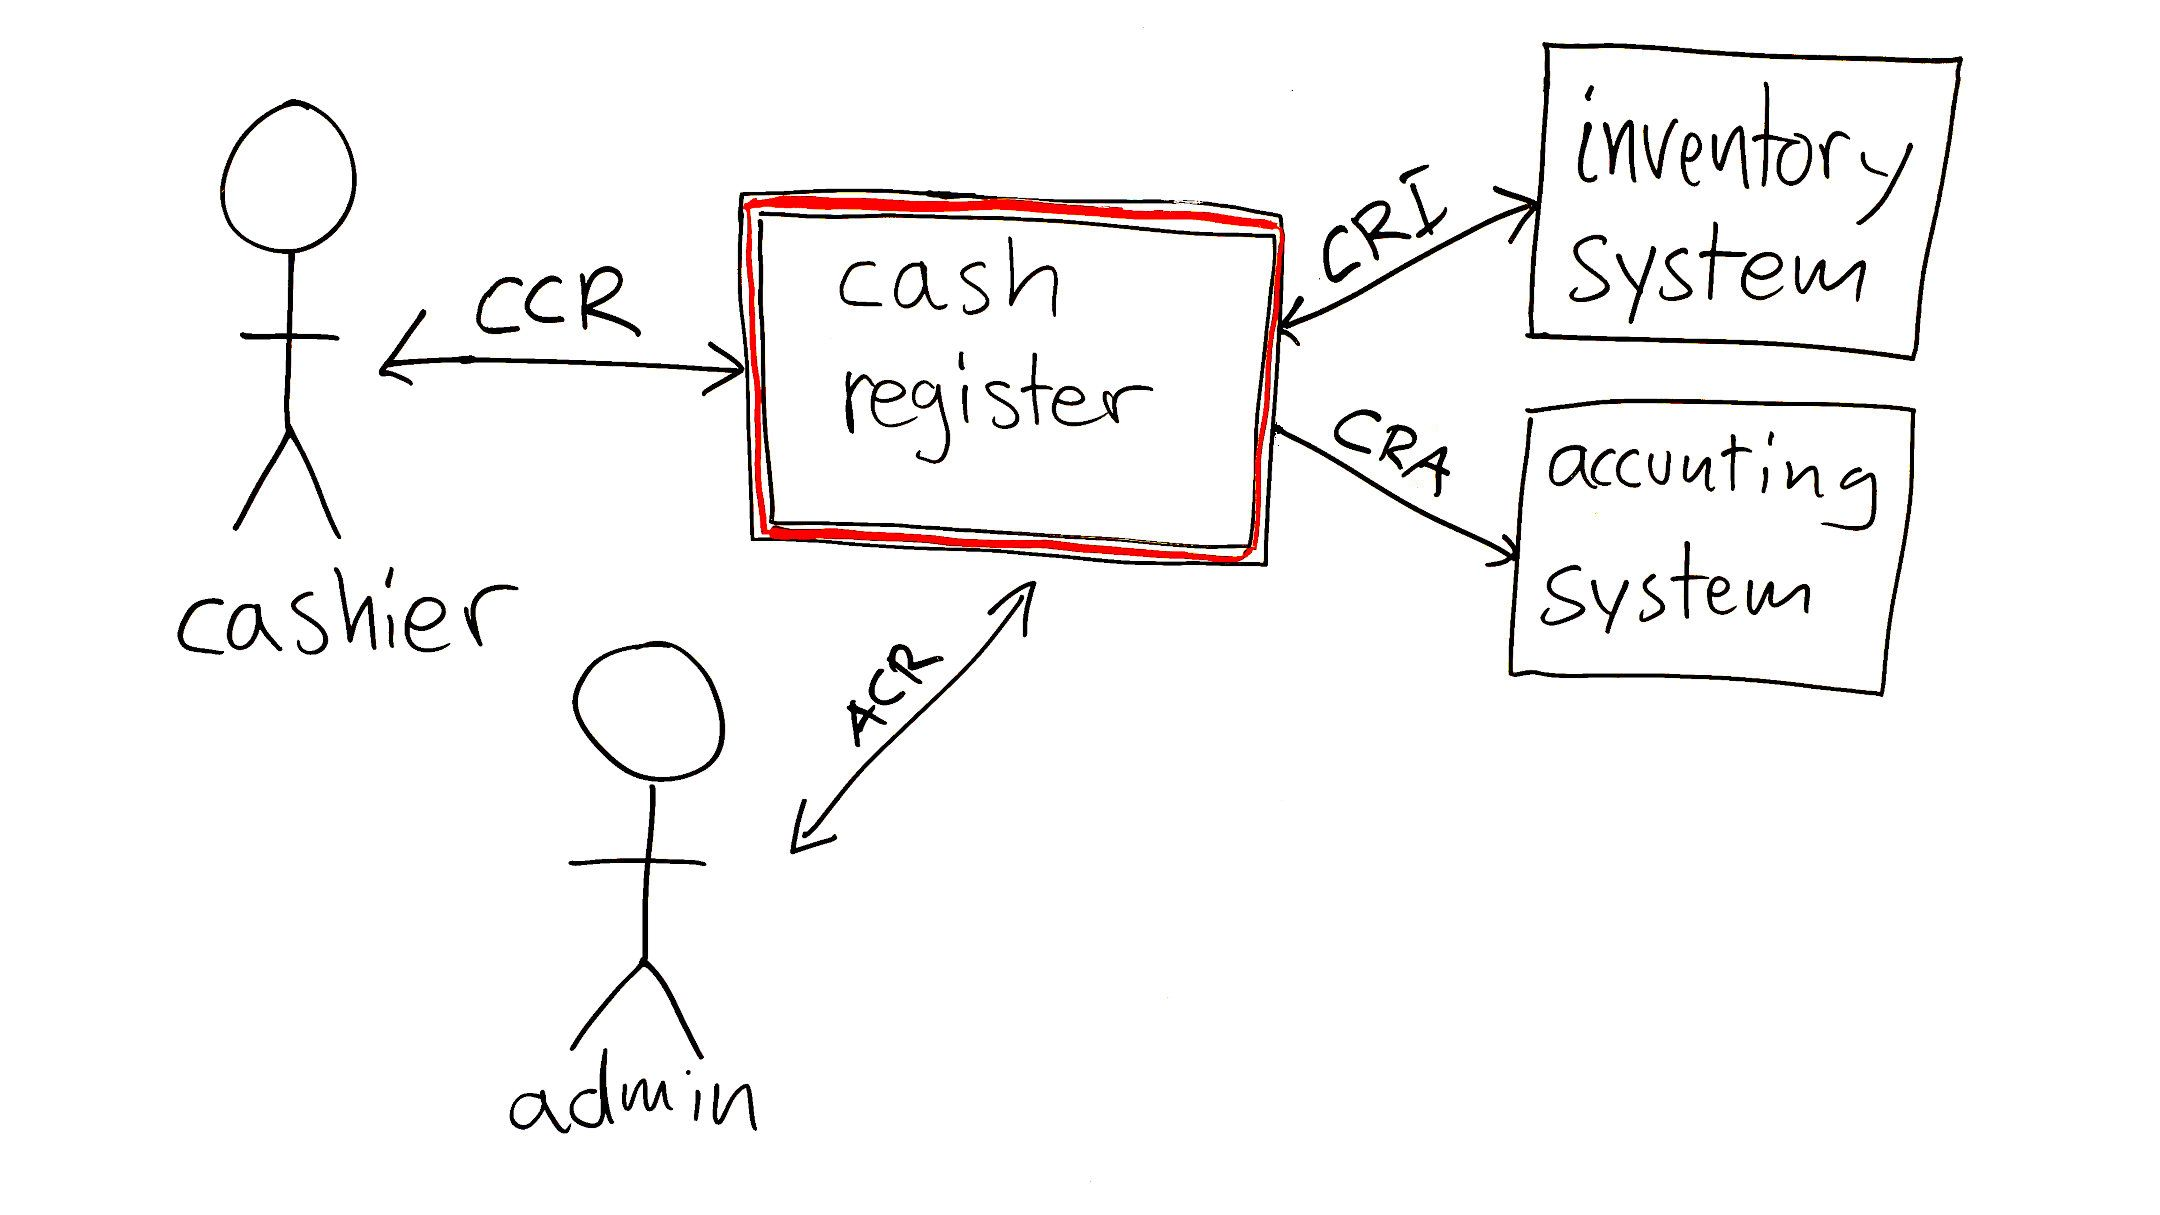
\includegraphics[width=0.9\textwidth]{../img/context-diagram-example}
\end{minipage}%
\vspace{1em}
\texttt{*~Interface~CRA}:\\ 
  \texttt{~~*~Spec:~The system shall ...~data entities ...}
\end{Slide}


\LectureOnly{\section{Elicitation}}

\begin{Slide}{Elicitation}

\begin{itemize}
\item \TODO{}

\end{itemize}
\end{Slide}

\LectureOnly{\section{Prioritization}}

\begin{Slide}{Prioritization}
Hello
\end{Slide}
* \TODO{}
\end{document}